%スタイル,パッケージの設定
\documentclass[12pt,a4]{jreport}%chapterが使えるスタイル
\usepackage[dvipdfmx]{graphicx}%図の挿入のためのパッケージ
\usepackage{amsmath}
\usepackage{setspace}
\usepackage{amssymb}
\usepackage{ascmac}
\usepackage{framed}

%余白の設定
\setlength{\textheight}{\paperheight}
\setlength{\topmargin}{4.6truemm}
\addtolength{\topmargin}{-\headheight}
\addtolength{\topmargin}{-\headsep}
\addtolength{\textheight}{-60truemm}
\setlength{\textwidth}{\paperwidth}
\setlength{\oddsidemargin}{-0.4truemm}
\setlength{\evensidemargin}{-0.4truemm}
\addtolength{\textwidth}{-50truemm}

%参考文献の設定
\renewcommand{\bibname}{参考文献}


%行間
\setstretch{1.4}

%表紙
\title{卒業論文\\Mg-LPSO の Small Cluster の第一原理計算}
\author{関西学院大学 理工学部\\情報科学科 西谷研究室\\3539 山本 泰基}
\date{2017年3月}
\begin{document}
\maketitle
\newpage

%概要
\begin{abstract}

LPSO ( Long Period Stacking Order ) 構造をもった Mg は比降伏強度でジュラルミンを上回る特性を持ち, かつ難燃性であるため次世代の航空機の構造材料として国内外から注目を集めている. LPSO 構造は, 母相 hcp 構造の [0001] 方向に対して周期的に積層欠陥が導入されることで長周期性を有する構造である.

西谷研究室では, この LPSO 構造の生成機構として「積層欠陥部に L1$_2$ クラスターが形成され, そこから排斥された Zn, Y が, 濃化して新たな L1$_2$ クラスターを形成する」というシナリオを立てた. このシナリオの実現性について, 第一原理計算を用いて評価してきた. 第一原理計算は, 量子力学を支配するシュレディンガー方程式を精確に解いて, 原子の種類だけから電子構造を求め, いろいろな物性を予測する計算である. 計算の結果, 系全体のエネルギーは溶質原子と L1$_2$ クラスターとの距離が離れるにつれ単調に減少し安定となった. しかしそれは中周期的に溶質原子が濃化するという LPSO の構造から予想される結果に反するものであった.

本研究では, 「 Small Cluster と L1$_2$ クラスターの相互作用」および「空孔を含んだクラスターの安定性」に関して第一原理計算をおこなった.「 Small Cluster と L1$_2$ クラスターの相互作用」に関して計算をおこなった結果, 4 層から 5 層離れた位置でエネルギーが最安定である結果が得られた. この結果は Small Cluster が積層欠陥部から中距離離れた位置で安定化するというシナリオを支持した.「空孔を含んだクラスターの安定性」に関しては Small Cluster から 3 層離した位置に空孔を挿入したモデルが最安定であった. これは, Small Cluster の周りに空孔が吸着し, クラスター拡散が誘発されるという仮説に反するものであった.
 \end{abstract}

%目次
\tableofcontents

%本文
\chapter{序論}


\section{Mg合金}
マグネシウム(Mg)は実用金属中において最も軽量かつ最大の振動吸収性をもつため, 航空機や自動車, 鉄道車両のフレーム, 工作機械で使用されるプーリーやロボットの骨格への応用が進められている. また,  Mg は海水中のにがりの主成分として含まれており日本国内においても十分に自給可能な金属である. このようなことから近年注目を集め, 様々な Mg 合金の研究開発が進められている. しかし,水やアルコールとよく反応してしまうため耐食性が悪く, Mg は 550 〜 600 °Cで発火するため大気中で火がつく可能性がある. それゆえ, 軽量金属であるアルミニウム(Al)合金に比べて実用が進んでいなかった.
しかし近年, Mg 合金において, LPSO 構造という新たな原子配列構造を持つ合金が開発され\cite{Th}, この Mg 合金は超々ジュラルミンの 1.2 倍の比降伏強度で, かつ難燃性であるという従来の常識を覆すような特性が得られている.


\section{LPSO 構造}
\subsection{積層欠陥}
積層欠陥とは, 積層順序の連続性が局所的に乱れた欠陥である. 図 1.1 に hcp 構造の積層欠陥の様子を表した模式図を示した. hcp 構造ではこの図で示すように [0001] 方向に最密面が ABAB と積層しており, 赤枠で囲った原子を赤矢印の方向にずらすと, 積層順序が ABCA となる. その際に赤の破線で示した部分が積層欠陥面となる. そして hcp 構造上に発生した積層欠陥面の上下の黄丸で示した層を中心とした積層順序を考えると, それぞれ ABC,BCA となっている. このことから hcp 構造において積層欠陥が発生すると cubic 構造である fcc 構造が導入されることがわかる.

\begin{figure}[htbp]
	\begin{center}
		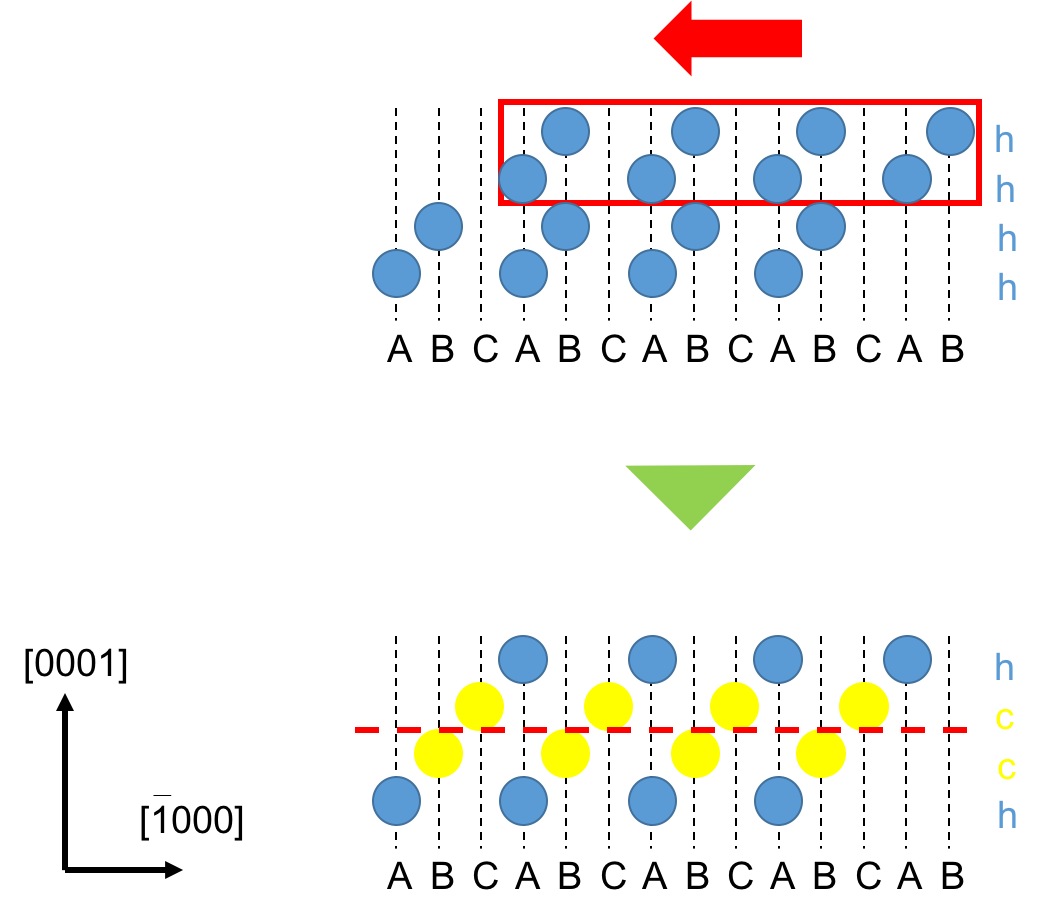
\includegraphics[width=100mm]{../intro/stuc.png}
		\caption{hcp 構造の積層欠陥の様子を表した模式図. 青丸は hexgonal 構造, 黄丸は cubic 構造を示している. また赤の破線部は積層欠陥部を示している.}
		\label{default}
	\end{center}
\end{figure}

\subsection{LPSO構造}
LPSO構造はその名称が示す通り,長周期の積層欠陥を含んだ構造であり,その積層欠陥部に溶質原子が濃化していることが研究の初期に判明していた. しかし, 液相から直接生成する合金系や, 固相から時効析出によって生成する系など多くの系で微妙に異なる構造を示すことが報告された. LPSO-Mg では下記の特徴がある.\\
\\(a) [0001] 方向において中周期的に積層欠陥が導入されている.\\
(b) 積層欠陥部には溶質原子であるZn,Yが集まっている.\\
(c) 集まった溶質原子が積層欠陥部において L12 型クラスターを形成している.

\subsection{LPSO構造生成シナリオ}
西谷研究室では, 生成メカニズムに関するシナリオを立て, それらの実現可能性を第一原理計算によりエネルギー的に検証してきた.当初は,
\\□積層欠陥先行型
\\  ・hcp 構造の Mg において, 周期的に積層欠陥が導入される.
\\  ・積層欠陥に溶質原子が捕まる.
\\□溶質原子先行型
\\  ・積層欠陥が溶質原子を捕まえる.
\\  ・積層欠陥から4層ほど離れた位置で溶質原子が濃化する.
\\  ・濃化した溶質原子が新たな積層欠陥を誘起する.\\
という2つのシナリオが立てられた.\\

\section{拡散}
\subsection{空孔拡散}
結晶中には原子の存在しない格子点があり, これを空孔(vacancy)という. 空孔と隣接する原子が位置を交換することにより拡散が起こる.
完全なカバレッジに近づく高いカバレッジレベルでの表面拡散の主な方法として起こり得る. このプロセスは、スライディングパズルで周りを滑るような方法に似ている. 高い拡散速度と低い空孔濃度のために、空孔拡散を直接観察することは非常に困難である. また, 単空孔と複空孔の拡散の模式図を図1.2, 図1.3に示した. 単空孔よりも複空孔の方が拡散の可能性が高くなる. それは図1.2で示した, 赤線の山(activation barrier)が単空孔のほうが高いのが原因である.

\begin{figure}[htbp]
	\begin{center}
		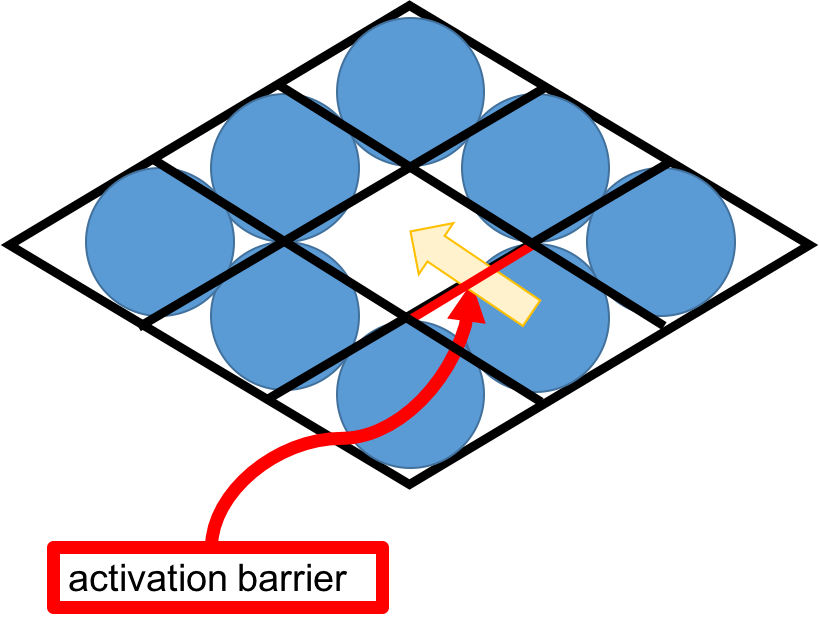
\includegraphics[width=80mm]{../intro/monovacancy.png}
        \caption{単空孔の拡散の模式図.}
		\label{default}
	\end{center}
\end{figure}

\begin{figure}[htbp]
	\begin{center}
		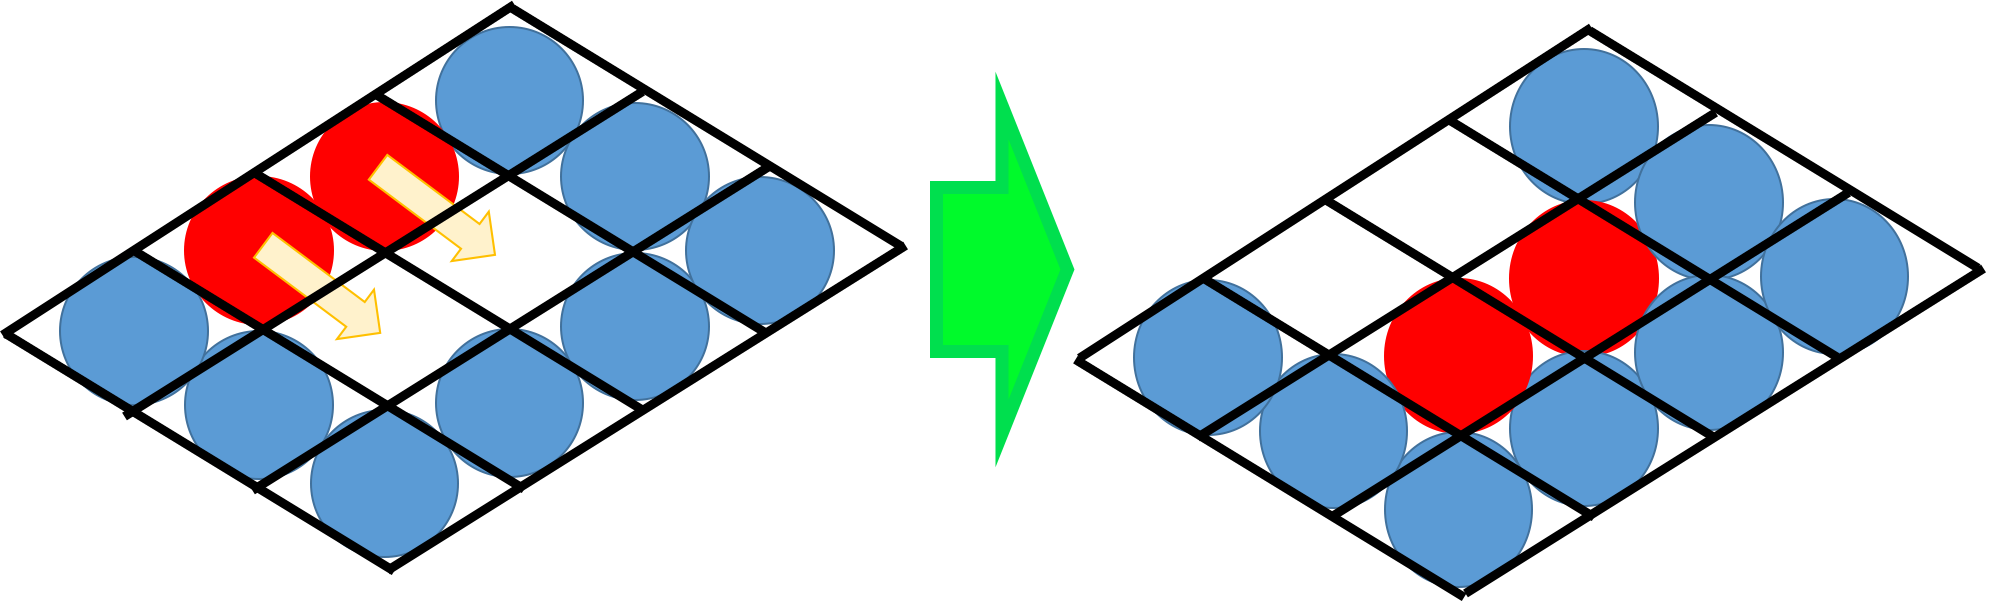
\includegraphics[width=130mm]{../intro/divacancy.png}
        \caption{複空孔の拡散の模式図.}
		\label{default}
	\end{center}
\end{figure}


\subsection{クラスター拡散}
クラスター拡散とは二原子から何百もの原子の塊の移動のことを言う。クラスターの動きは、個々の原子、クラスターのセクション、またはクラスタ全体が移動する場合がある。
クラスター拡散に関して, 結晶の表面では可能であるが, バルクでは不可能である.
理由は表面では上が空いているので動くことが可能だが(図1.4), バルクでは上も原子が詰まっており動くことができないからである(図1.5).

\begin{figure}[htbp]
	\begin{center}
		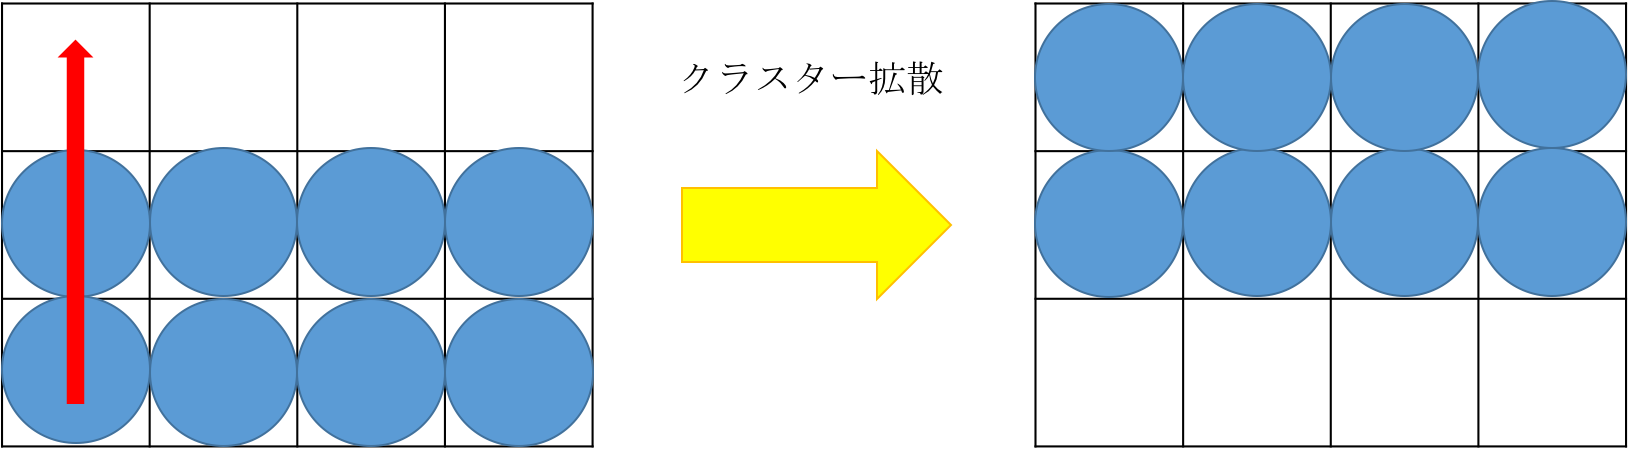
\includegraphics[width=100mm]{../intro/kakusan.png}
		\caption{クラスター拡散の模式図.}
		\label{default}
	\end{center}
\end{figure}

\begin{figure}[htbp]
	\begin{center}
		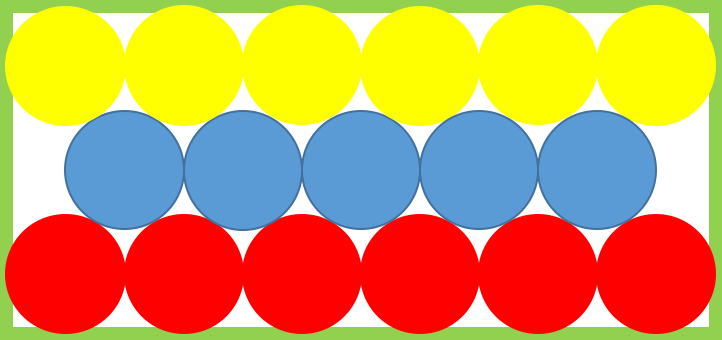
\includegraphics[width=70mm]{../intro/balc.png}
        \caption{バルク内の模式図.}
		\label{default}
	\end{center}
\end{figure}

\section{構造緩和}
構造緩和とは, 原子, または原子の集団を移動させて, 最安定構造を見つける事である. 本研究で行う構造緩和は, 結晶中の各原子を個々に移動させる内部緩和と, 格子定数を変化させて結晶格子の構造自体を緩和させる外部緩和を用いて, 最安定構造を求め, エネルギー値を算出する.

%序論
\chapter{手法}


\section{第一原理計算}
第一原理計算とは, シュレディンガー方程式を精確に解いて, 原子の種類だけから電子構造を求め, 様々な物性を予測する計算である. しかし, 第一原理計算は非常に高い精度が要求される複雑なものである.


\section{VASP}
VASP (Vienna Ab-initio Simulation Package) は, 密度汎関数理論による平面波・擬ポテンシャル法を用いた第一原理計算プログラムパッケージである. 密度汎関数理論とは電子系等のエネルギーなどの物性は電子密度から計算できるという理論である. 擬ポテンシャル法とは原子の内殻電子を除いた価電子だけを考慮する手法であり, 全電子を計算するフルポテンシャル法に比べ比較的高速な計算が可能となるため, 擬ポテンシャル法であっても十分な精度で計算ができる.
VASP の計算には, 計算条件が記述された INCAR, 計算モデルの構造が記述された POSCAR, 原子情報が記述された POTCAR, 計算精度を司る k−mesh が記述された KPOINTS の 4 種類の入力ファイルを使用し計算を行う. その後, 計算モデル内における原子の安定位置やフォース, 系の全体エネルギー等が記述された OUTCAR 等を出力する.


\section{計算モデル}
\subsection{周期的境界条件}
VASP で計算を行う場合, 平面波を用いた第一原理計算が行われるため, 無限周期の固体を考えなければならないが計算モデル内の原子が増えるにつれ計算時間も増えるため, 無限周期のモデルの計算を行うことはできない. そこで図 2.1 のように同じモデルが全方向に無限に隣接したようなモデルを考える. このモデルであれば, 無限周期の固体と見なせるため平面波を考慮することができる. このような計算条件を周期的境界条件という.

\begin{figure}[htbp]
	\begin{center}
		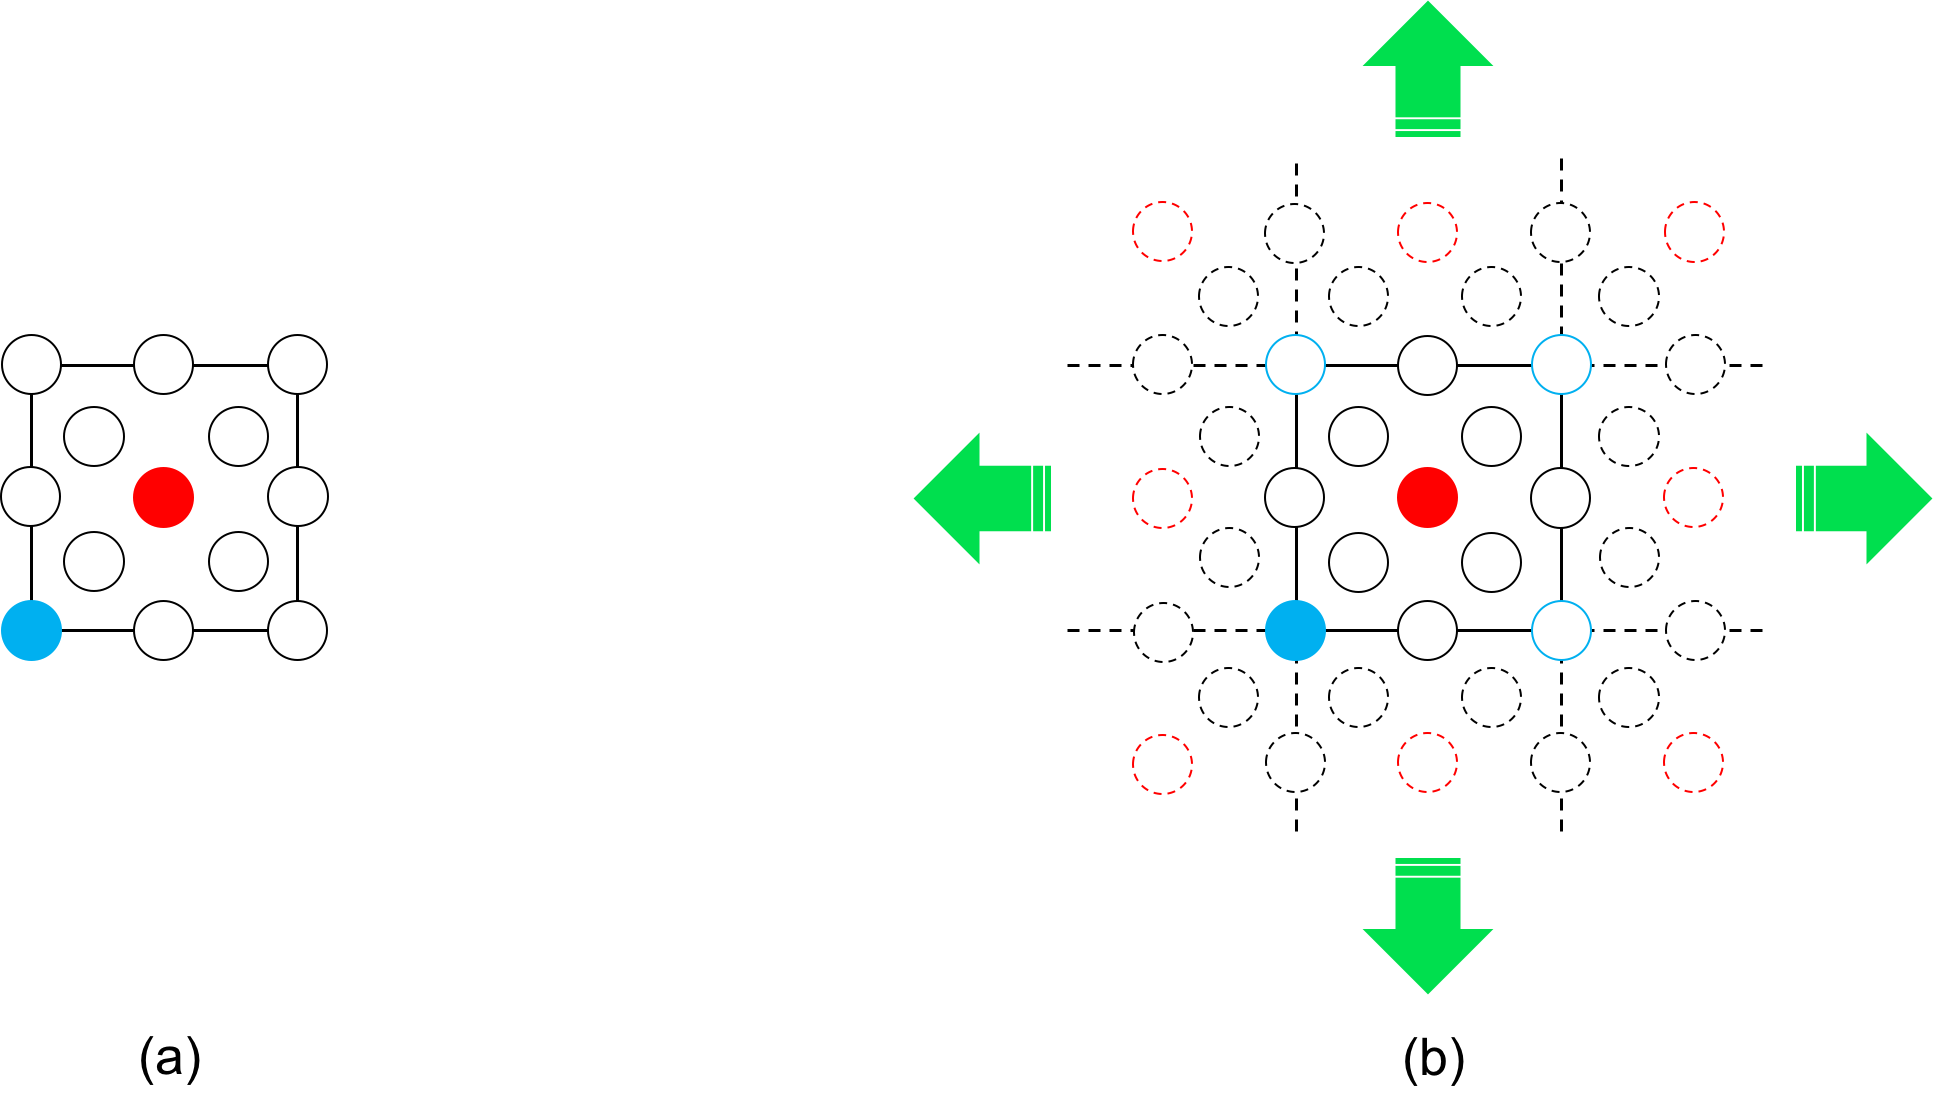
\includegraphics[width=130mm]{../method/cnd.png}
		\caption{(a) 周期的境界条件を考慮しないモデルの模式図.(b) 周期的境界条件を考慮したモデルの模式図.実線部分は計算モデル,破線部分は隣接した計算モデルを表している.}
		\label{default}
	\end{center}
\end{figure}


\subsection{ L1$_2$ クラスターおよび Small Cluster の導入}
清原らは,L12 クラスターを hcp 構造に強引に導入すると, 図2.2の (a), (b) のように縦方向と横方向の 2 つに分裂した集団が生成すると予測している\cite{kiyohara}. このサイズは実験的には奥田らが報告しているクラスターサイズに近い\cite{okuda}. 

\begin{figure}[htbp]
	\begin{center}
		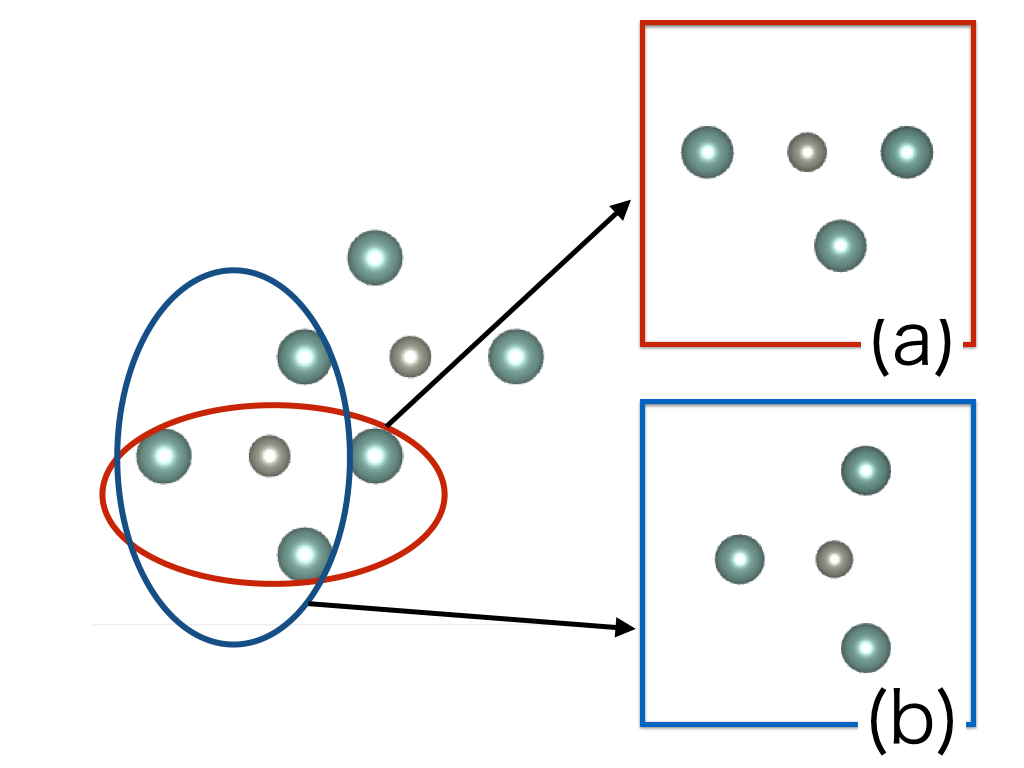
\includegraphics[width=50mm]{../method/MiniCluster.png}
		\caption{Small Cluster の模式図.}
		\label{default}
	\end{center}
\end{figure}

これらの集団を 6層の Mg 結晶に導入したモデルについて検証した. 系全体のエネルギーを第一原理計算により求めた結果, (a) のモデルが安定であるという結果が得られた. 今回, 本研究では (a) を Small Cluster とした. 西谷研究室では, Small Cluster と L1$_2$ クラスターの相互作用の計算モデルは, 必要最小の原子数でしか行っていなかった. そのため, Small Cluster も周期的に並んだモデルとなっている. より現実的なモデルとしては, 隣接する Small Cluster との相互作用の影響が及ばないだけの距離をとるサイズで計算する必要がある. そこで, 24層の slub モデルを構築し, Small Cluster を図 2.3 のように L1$_2$ クラスターから Small Cluster を1層ずつ離した slab モデルに挿入して, VASP を用いて第一原理計算を行い, 構造緩和したエネルギーを求めた.

\begin{figure}[htbp]
	\begin{center}
		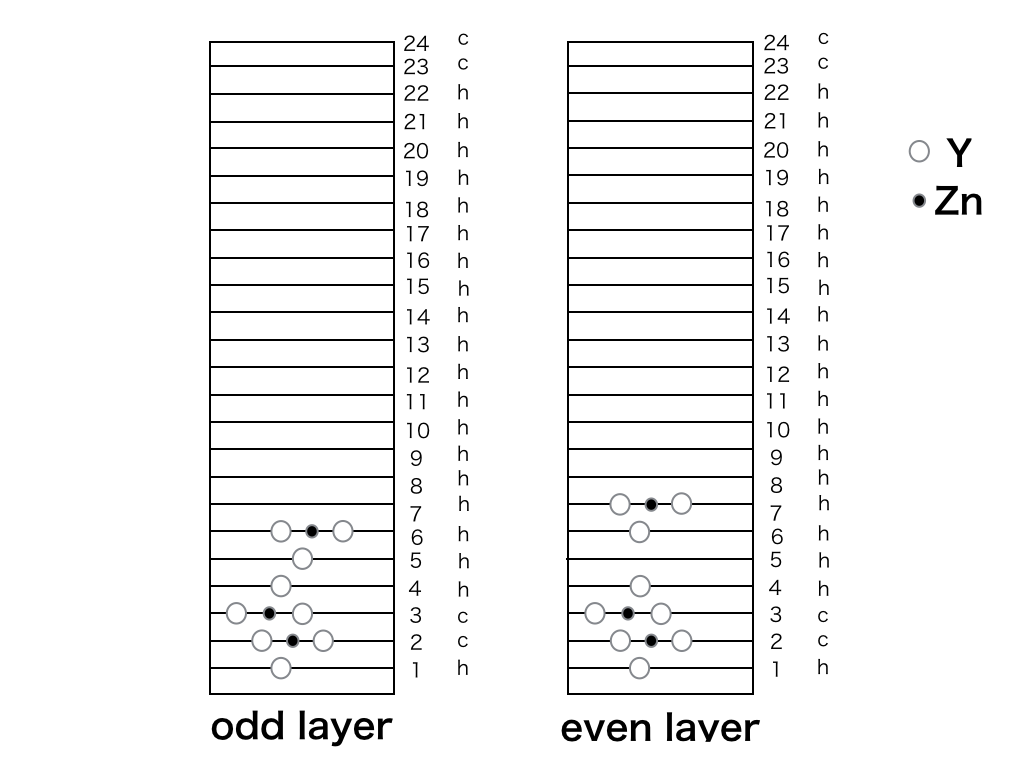
\includegraphics[width=80mm]{../method/small_cluster_slab.png}
		\caption{slub モデルの模式図.}
		\label{default}
	\end{center}
\end{figure}


\subsection{ Small Cluster および 空孔の導入}


\section{Small Cluster と空孔の挿入位置}
L1$_2$ クラスターを導入したモデルに Small Cluster や空孔を挿入するには様々な配置パターンがあり, すべての配置を考慮するのは困難である. そこで, 西谷研究室では, 各配置 場所に a から順に番号を振り分ける方法を用い, 各層での配置パターンを決定した. L1$_2$ クラスターから 1, 3, 5 …層離れた層は C 層, 2, 4 …層離れた層は A 層の配置となっている. アルファベットの組み合わせの模式図を図 2.4 で示した. また, 赤, 青, 緑, 黄丸はそれぞれ L1$_2$ クラスターから第 0~3 近接原子を表している.

\begin{figure}[htbp]
    \begin{tabular}{cc}
      \begin{minipage}{0.5\hsize}
        \centering
        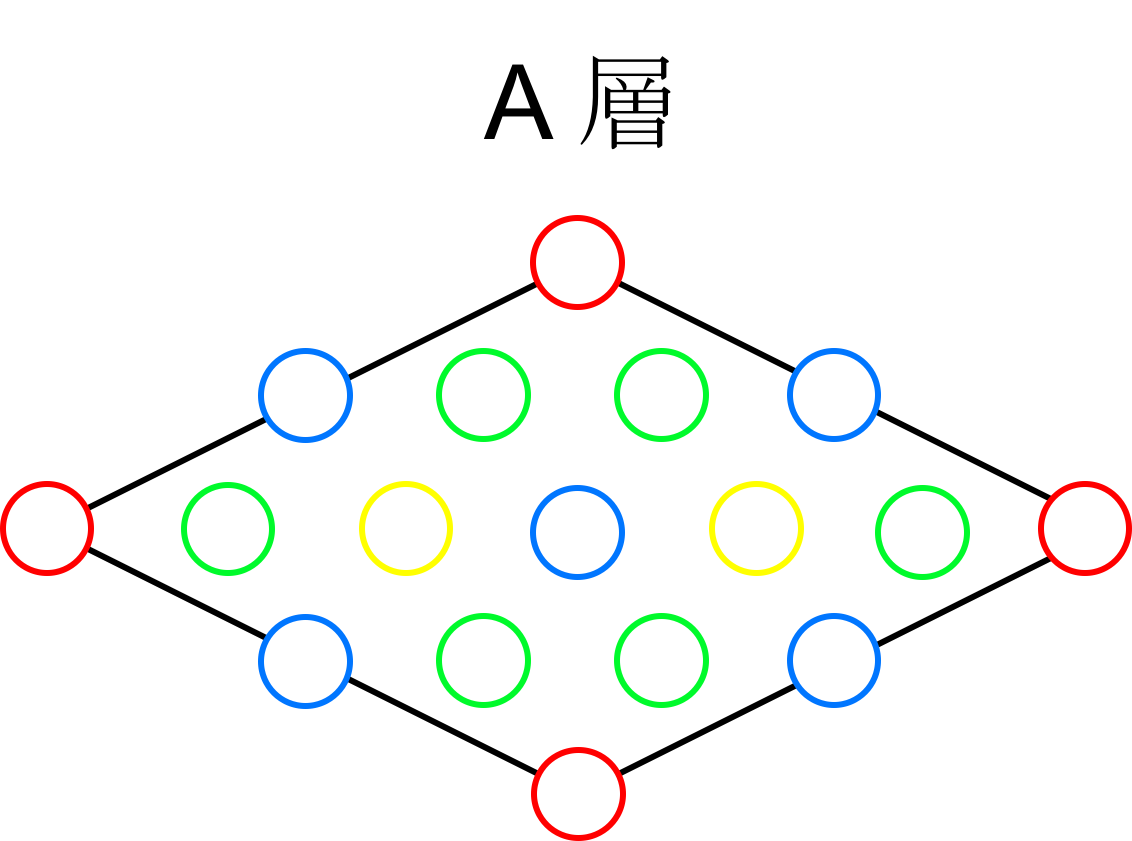
\includegraphics[width=80mm]{../method/Alayer.png}
        \label{default}
      \end{minipage} &
      \begin{minipage}{0.5\hsize}
        \centering
        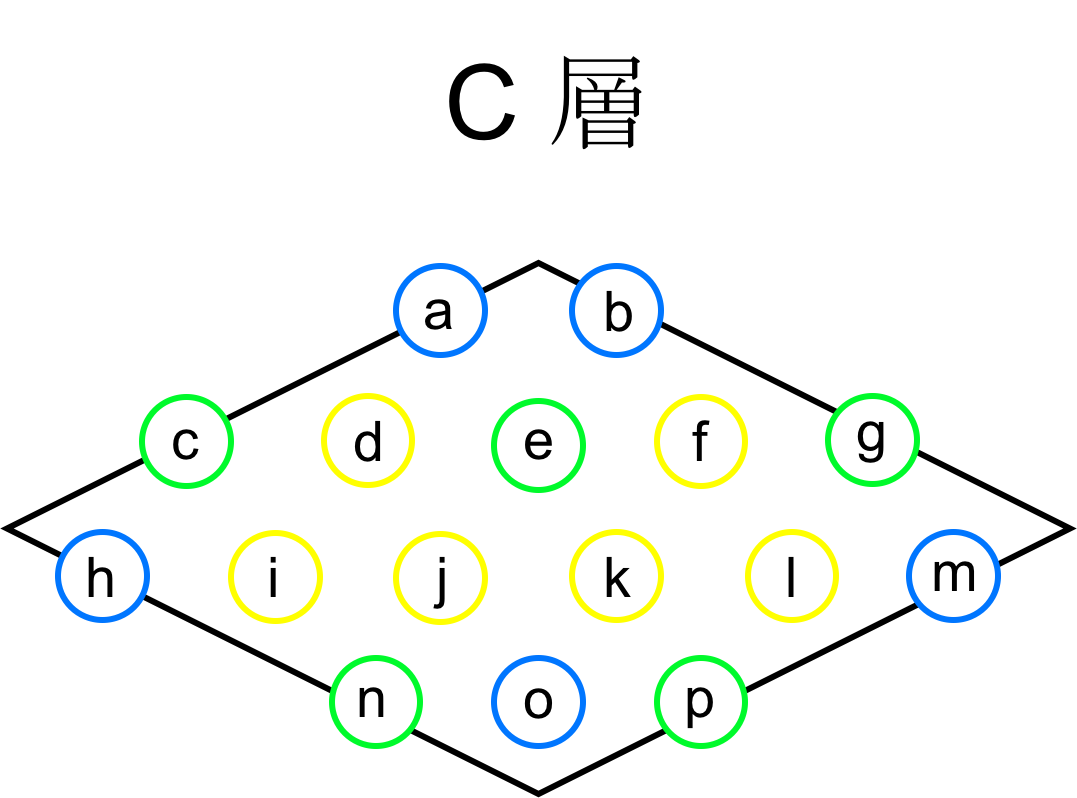
\includegraphics[width=80mm]{../method/Clayer.png}
        \label{default}
      \end{minipage}
    \end{tabular}
    \begin{center}
		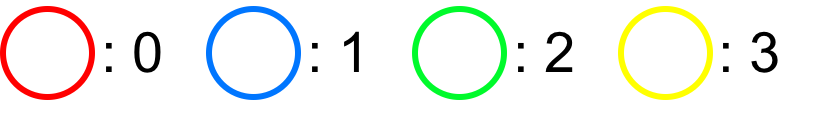
\includegraphics[width=50mm]{../method/AClayer.png}
		\caption{配置パターンの模式図.}
		\label{default}
	\end{center}
  \end{figure}




%手法
\chapter{結果}
\section{ L1$_2$ クラスターおよび Small Cluster の導入}

\subsection{18層の slub モデルの計算結果}

18層の slub モデルの系全体のエネルギーの計算結果をまとめたグラフを図\ref{fig18} に示す. 18 層の計算では, 4 層の計算が収束しなかった. しかし, わずかではあるがエネルギー傾向が 5層から 7層で単調増加を示した. このままエネルギーが増加を示すと別の L1$_2$ クラスターから影響を受けている事を示唆する. 8層以降で増加が止まれば別の L1$_2$ クラスターからの影響ではなく Small Cluster が中距離で安定するという事が示唆される. しかし, それ以降の値が判明していなかったために, 8 層以降のエネルギー傾向が単調増加するかどうかが判明しなかった.

\begin{figure}[htbp]
	\begin{center}
		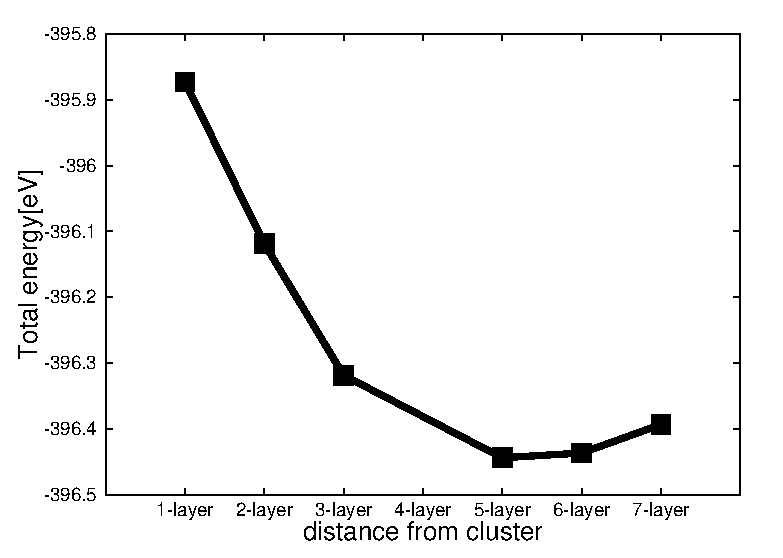
\includegraphics[width=100mm]{../result/small_cluster.eps}
		\caption{18層の slub モデルのエネルギー.}
		\label{fig18}
	\end{center}
\end{figure}

\subsection{C 層に Small Cluster を挿入した時のエネルギー}
クラスターから 1, 3, 5, 7, 9 層離れた層は C 層の原子配置であり, 図\ref{fig3.1} で示す. ここでは青丸は第 1 近接位置, 緑丸は第 2 近接位置, 黄丸は第 3 近接位置を表している. 表3.1 は C 層の第 1, 2, 3 近接距離に Small Cluster を挿入したモデルのエネルギーを表している.

\begin{figure}[htbp]
	\begin{center}
		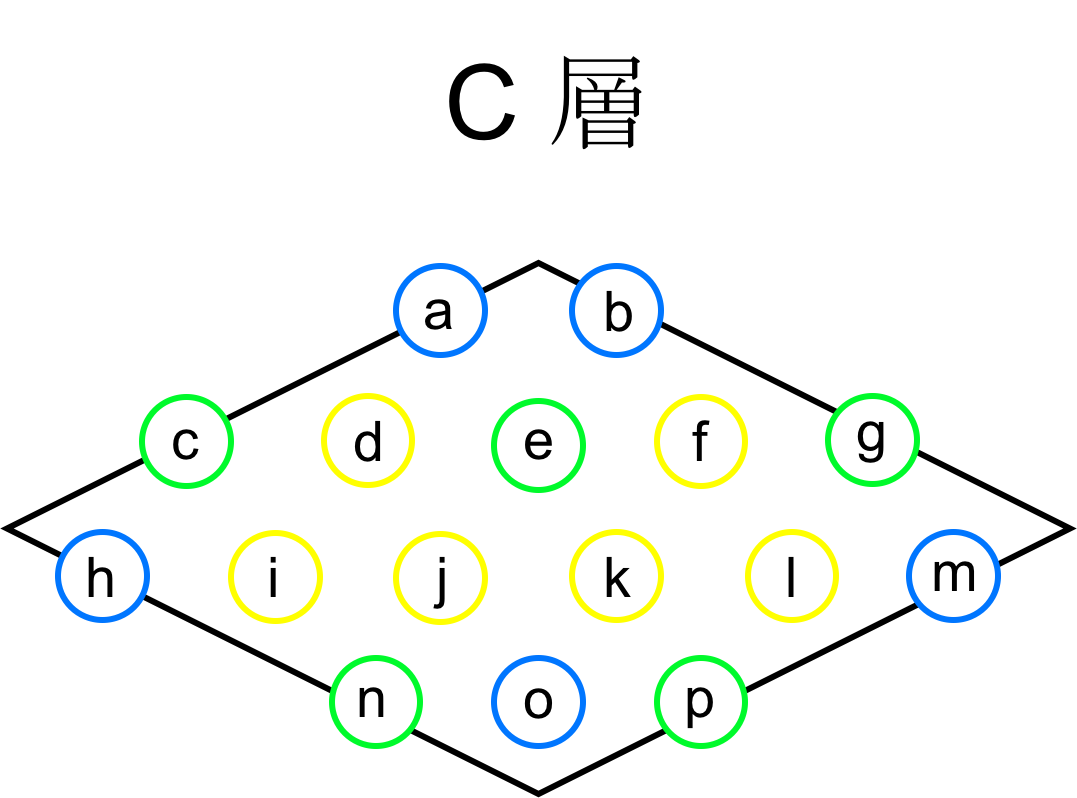
\includegraphics[width=90mm]{../method/Clayer.png}
		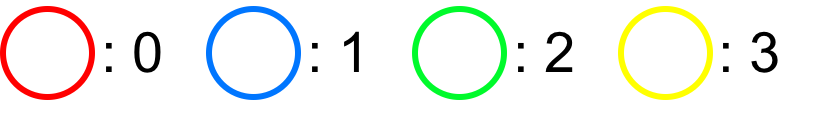
\includegraphics[width=60mm]{../method/AClayer.png}
		\caption{C 層の第 0, 1, 2, 3 近接位置を表した模式図.}
		\label{fig3.1}
	\end{center}
\end{figure}

\begin{table}[H]
\caption{C 層の第 1, 2, 3 近接距離に Small Cluster を挿入したモデルのエネルギー [eV].}
  \begin{center}
    \begin{tabular}{|l|c|c|c|c|c|} \hline
         & 第 1 層 & 第 3 層 & 第 5 層 & 第 7 層 & 第 9 層\\ \hline
第 1 近接位置 & -506.773098 & -507.223404 & -507.339844 & -507.300403 & -507.274385\\
\hline
第 2 近接位置 & -506.872873 & -507.240530 & -507.340992 & -507.305620 & -507.279716\\
\hline
第 3 近接位置 & -506.975043 & -507.255849 & -507.342078 & -507.300835 & -507.273358\\
\hline
    \end{tabular}
  \end{center}
\end{table}


\subsection{A 層に Small Cluster を挿入した時のエネルギー}
クラスターから 2, 4, 6, 8, 10 層離れた層は A 層の原子配置であり, 図\ref{fig3.2} で示す. ここでは赤丸は第 0 近接位置, 青丸は第 1 近接位置, 緑丸は第 2 近接位置, 黄丸は第 3 近接位置を表している. 表3.2 は A 層の第 0, 1, 2, 3 近接距離に Small Cluster を挿入したモデルのエネルギーを表している.

\begin{figure}[htbp]
	\begin{center}
		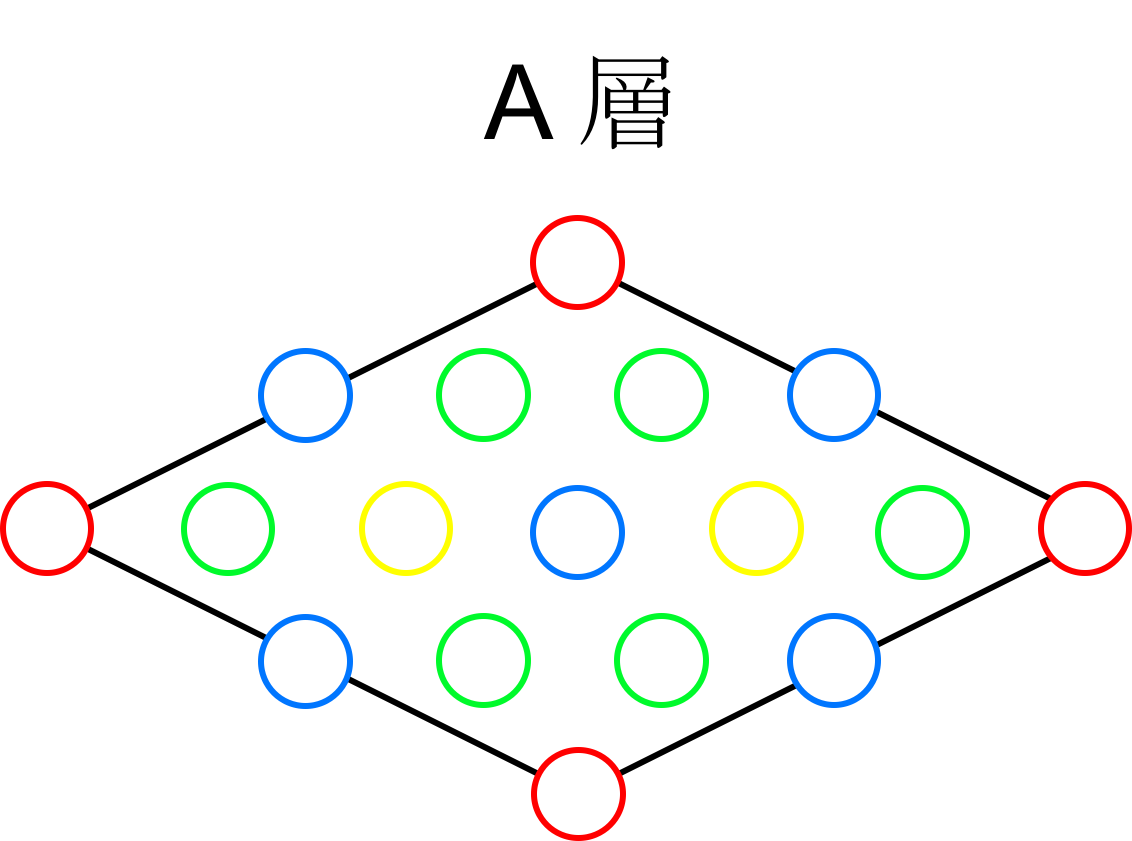
\includegraphics[width=90mm]{../method/Alayer.png}
		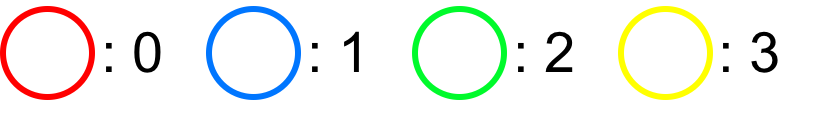
\includegraphics[width=60mm]{../method/AClayer.png}
		\caption{A 層の第 0, 1, 2, 3 近接位置を表した模式図.}
		\label{fig3.2}
	\end{center}
\end{figure}

\begin{table}[H]
\caption{A 層の第 0, 1, 2, 3 近接距離に Small Cluster を挿入したモデルのエネルギー [eV].}
  \begin{center}
    \begin{tabular}{|l|c|c|c|c|c|} \hline
         & 第 2 層 & 第 4 層 & 第 6 層 & 第 8 層 & 第 10 層\\ \hline
第 0 近接位置 & -507.041788 & -507.340218 & -507.324580 & -507.264994 & -507.274057\\
\hline
第 1 近接位置 & -507.095924 & -507.313473 & -507.327796 & -507.279462 & -507.274801\\
\hline
第 2 近接位置 & -507.117741 & -507.307283 & -507.334387 & -507.283037 & -507.272749\\
\hline
第 3 近接位置 & -507.152164 & -507.348526 & -507.336189 & -507.273986 & -507.275103\\
\hline
    \end{tabular}
  \end{center}
\end{table}

図\ref{fig3.3} は表 3.1 と表 3.2 のエネルギー値をグラフにまとめたものである. 赤点は第 0 近接位置, 青点は第 1 近接位置, 緑点は第 2 近接位置, 黄点は第 3 近接位置のエネルギーである.

\begin{figure}[htbp]
	\begin{center}
		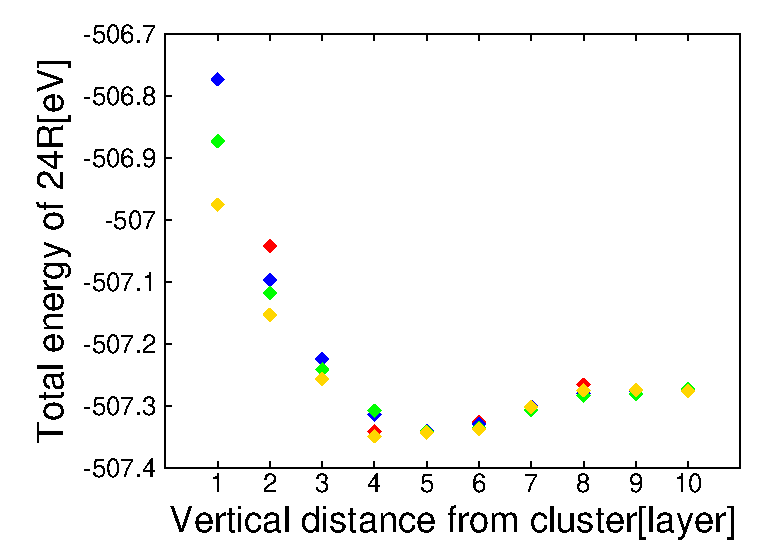
\includegraphics[width=90mm]{../result/small_cluster_Alld_color.eps}
		\caption{各層のエネルギーをまとめたグラフ.}
		\label{fig3.3}
	\end{center}
\end{figure}


\section{ Small Cluster および 空孔の導入}
1層12原子として, 6層の純粋な hcp-Mg 結晶がもつ系全体のエネルギーは -249.815039 eV である. 空孔を含む 6 層の Mg 結晶の系全体のエネルギーは -247.517691 eV である. これらの計算結果から空孔の形成エネルギーを算出した. 空孔の形成エネルギーの計算方法は以下の通りである.

\begin{enumerate}
 \item 純粋な Mg 結晶の結果から, hcp-Mg 1個が持つエネルギーを算出.\\ -249.815039/162;\\
-1.542068142
 \item 1 個のエネルギーから本来の Mg 161 個が持つエネルギーを算出.\\
-1.542068142*161;\\
-248.2729709
 \item 2 項目で得られた値とincludeの値の差を計算.\\
-248.2729709-(-247.517691);\\
-0.7552799
\end{enumerate}
これがこれが空孔の形成エネルギーである.


図\ref{fig2.4} のモデルにおいて, 空孔を挿入したモデルのエネルギーを表 3.3に示す.

\begin{table}[htb]
\caption{空孔を挿入した時のエネルギー.}
  \begin{center}
    \begin{tabular}{|l|c|c|c|c|c|} \hline
 挿入位置 & エネルギー [eV] \\ \hline
   (a) & -268.452640\\
\hline
   (b) & -267.932411\\
\hline
   (c) & -268.496561\\
\hline
    \end{tabular}
  \end{center}
\end{table}
%結果
\chapter{考察}

1. Zn-Y ペアが 積層欠陥が導入されている 同層に捕まる .
2. 濃化した溶質原子が 積層欠陥を誘起する .
3. 積層欠陥が溶質原子を 捕まえる .
4. 積層欠陥ができた層で クラスターが形成される .
5. Zn と Y の両原子が共に 積層欠陥から掃き出される .
6. 4 層程度離れた位置で 溶質原子が濃化する .
7. 2-6 の行程を繰り返す .%考察
\chapter{総括}
%総括
\chapter*{謝辞} 
本研究を進めるにあたり,終始多大なるご指導,細部にわたって有益な助言と指導をいただきました西谷滋人教授に対し,厚く御礼申し上げます.また,本研究の進行に伴い,
様々な助力を頂きました西谷研究室の同輩,先輩方に心から感謝の意を表します.%謝辞

%参考文献

\begin{thebibliography}{9}
\bibitem{Th}Y. Kawamura, K. Hayashi, A. Inoue and T. Masumoto: Mater. Trans., 42, 1172(2001).

\bibitem{kiyohara} M. Kiyohara, Y. Sakamoto, T. Yoshioka, S. Morishita, and S. R. Nishitani: proceedings of PRICM9, (Kyoto 2016).

\bibitem{okuda} H. Okuda, M. Yamasaki, Y. Kawamura, M. Tabuchi, H. Kimizuka: Scientific Reports, {\bf5} (2015), 14186.
\end{thebibliography}

\end{document}
%終了